\RequirePackage[l2tabu,orthodox]{nag}
\pdfoutput=1
\pdfminorversion=3
\documentclass[compress]{beamer}\usetheme{Warsaw}\usecolortheme{crane}\useoutertheme[subsection=false]{smoothbars}
\setbeamertemplate{navigation symbols}{}
\definecolor{links}{HTML}{2A1B81}
\hypersetup{pdfpagemode=FullScreen,colorlinks,linkcolor=,urlcolor=links}
\usepackage[english]{babel}
\usepackage{amsmath}
\usepackage{amssymb}
\usepackage{latexsym}
\usepackage{graphicx}
\usepackage{xcolor}
\usepackage{url}
\usepackage{listings}
\usepackage{multirow}
\usepackage{subfigure}
\usepackage{algorithmic}
\usepackage{tikz}
\usetikzlibrary{er}
\usetikzlibrary{shadows}
\tikzstyle{every attribute} = [top color=white, bottom color=yellow!40, drop shadow]

\title[Initial Foray into ML and Quantum-Enhanced Protocols]{Initial Foray into Machine Learning and Quantum-Enhanced Protocols}

\author{Quantum Machine Learning Reading Group @ ICFO}

\date{30 March 2017}

\subject{Talks}

\begin{document}
\frame[plain]{
  \titlepage
}

\section{Classical Machine Learning}
%%%%%%%%%%%%%%%%%%%%%%%%%%%%%%%%%%%%%%%%%%%%%%%%%%%%%%%%%%%%%%%%%%%%%%%
\begin{frame}{How do AI and machine learning relate?}
\begin{itemize}
	\item Better not draw Venn diagrams\ldots
	\item Roughly: deep learning $\subset$ machine learning $\subset$ AI.
	\item There is a good deal of overlap between statistical inference and machine learning.
	\item Between optimal control theory and machine learning: reinforcement learning.
\end{itemize}
\end{frame}

%%%%%%%%%%%%%%%%%%%%%%%%%%%%%%%%%%%%%%%%%%%%%%%%%%%%%%%%%%%%%%%%%%%%%%%
\begin{frame}{One possible categorization of schools of thought}
\begin{itemize}
 \item Connectionism: neural networks and empirical risk minimization.
 \item Structural risk minimization: support vector machines, regularized boosting\ldots
 \item Probabilistic inference: Bayesian and Markov networks.
 \item Symbolic AI: first-order logic or other form of formal reasoning.
\end{itemize}
\end{frame}

%%%%%%%%%%%%%%%%%%%%%%%%%%%%%%%%%%%%%%%%%%%%%%%%%%%%%%%%%%%%%%%%%%%%%%%
\begin{frame}{Statistics and sample complexity}
  \begin{itemize}
	  \item Descriptive and \textbf{inferential} statistics.
    \item Assumptions derive from probability theory.
    \item Parameters enter through assumed probability distributions.
    \begin{itemize}
      \item It is often assumed that the data is generated by \textbf{certain probability distributions} described by a finite number of unknown parameters.
    \end{itemize}
	  \item Law of large numbers.
    \begin{itemize}
       \item Concentration theorems.
    \end{itemize}
    \item Independent and identically distributed (IID) random variables.
    \item We can establish guarantees on accuracy based on the \textbf{sample size}.
    \item Example: metrology.
    \begin{itemize}
      \item Standard quantum limit: scales as $1/N$.
      \item Heisenberg limit: scales as $1/N^2$.
    \end{itemize}
  \end{itemize}
\end{frame}

%%%%%%%%%%%%%%%%%%%%%%%%%%%%%%%%%%%%%%%%%%%%%%%%%%%%%%%%%%%%%%%%%%%%%%%%%
\begin{frame}{Model complexity and parsimony}
\begin{itemize}
\item Aristotle (4th century B.C.): ``We may assume the superiority ceteris paribus [other things being equal] of the demonstration which derives from fewer postulates or hypotheses.''
\item Occam's razor (1300s): ``Among competing hypotheses, the one with the fewest assumptions should be selected.''
\item \textbf{Combinatorial explosion} in AI and uncertainty. The problem of \textbf{overfitting}.
\item Number of free parameters is insufficient to characterize the learning capacity of a function family (see hyperplanes versus the sine function).
\item Combinatorial measure of model complexity: VC dimension.
\item Control of model complexity: via \textbf{regularization} of the cost function. We usually use a convex regularization term that we can solve efficiently classically ($l_2$-norm: XGBoost \href{https://arxiv.org/abs/1603.02754}{(Chen \& Guestrin, 2016)} and the least-squares formulation of support vector machines in \href{https://arxiv.org/abs/1307.0471}{Rebentrost, Mohseni \& Lloyd, 2014}).
\end{itemize}
\end{frame}

%%%%%%%%%%%%%%%%%%%%%%%%%%%%%%%%%%%%%%%%%%%%%%%%%%%%%%%%%%%%%%%%%%%%%%%
\begin{frame}{The essence of statistical learning theory}
Elements of balance:
\begin{itemize}
 \item Sample complexity.
 \item Computational complexity.
 \item Model complexity.
\end{itemize}
\begin{block}{Generalization bounds}
\footnotesize{
$P\left(E(h) \leq E_S(h) + F(\textrm{model complexity of function family }\mathcal{H}, N, \eta)\right)\geq 1-\eta$}
\end{block}
\begin{itemize}
  \item $\mathcal{H}$ is the function family we optimize over.
  \item $F$ goes to zero as $N\rightarrow\infty$.
  \item $F$ monotonically increases with model complexity.
  \item IID assumption.
  \item $E(h)$ is the error of the learned function $h$ over the whole distribution given the sample.
  \item $E_S$ is the error on the sample, the training error, the empirical risk.
\end{itemize}
\end{frame}

%%%%%%%%%%%%%%%%%%%%%%%%%%%%%%%%%%%%%%%%%%%%%%%%%%%%%%%%%%%%%%%%%%%%%%%
\begin{frame}{What's an easy problem? What's a hard one?}
	From easier to harder:
	\begin{itemize}
		\item Supervised learning: this is where deep learning shines. See \href{http://doi.org/10.1038/nature14539}{LeCun et al., 2015}, \href{https://github.com/peterwittek/qml-rg\#meeting-5}{coding exercise for Meeting 5}.
		\item Semi-supervised learning.
		\item Unsupervised learning. E.g. autoencoders (\href{https://arxiv.org/abs/1612.01045}{Wan et al., 2016}; \href{https://github.com/peterwittek/qml-rg\#meeting-2}{coding exercise for Meeting 2}).
		\item Generative models.
		\item Reinforcement learning. See \href{http://doi.org/10.1038/nature16961}{Silver et al., 2016}, coding exercises for \href{https://github.com/peterwittek/qml-rg\#meeting-3}{Meetings 3} and \href{https://github.com/peterwittek/qml-rg\#meeting-4}{4}.
	\end{itemize}
\end{frame}

%%%%%%%%%%%%%%%%%%%%%%%%%%%%%%%%%%%%%%%%%%%%%%%%%%%%%%%%%%%%%%%%%%%%%%%
\begin{frame}{Why does deep learning work?}
\begin{itemize}	
	\item It has an enormous model complexity: the generalization bound does not seem to be tight.
	\item But:
	\begin{itemize}
		\item Massive amounts of labeled data are available, so $N$ is large. With \emph{data augmentation} (see coding exercises for \href{https://github.com/peterwittek/qml-rg\#meeting-5}{Meetings 5} and \href{https://github.com/peterwittek/qml-rg\#meeting-6}{6}), $N$ can be increased further.
		\item Massively parallel computational resources and matching toolkits became common place (see \href{https://arxiv.org/abs/1603.04467}{Abadi et al., 2016}; coding exercise for \href{https://github.com/peterwittek/qml-rg\#meeting-2}{Meeting 2} and all subsequent task with DL). Furthermore, research is extensive on improving optimization techniques for deep architectures (\href{https://arxiv.org/abs/1412.6980}{Kingma \& Ba, 2014}).
	\end{itemize}
	\item The layers take care of feature engineering that used to be the primary preoccupation of data scientists of yore (then called data miners). Compare the results you got with the various learning algorithms on the APS captcha exercise.
	\item Also: deep networks can be regularized (see the upcoming Meeting 7).
\end{itemize}
\end{frame}

%%%%%%%%%%%%%%%%%%%%%%%%%%%%%%%%%%%%%%%%%%%%%%%%%%%%%%%%%%%%%%%%%%%%%%%
\section{Quantum-Enhanced Learning}
%%%%%%%%%%%%%%%%%%%%%%%%%%%%%%%%%%%%%%%%%%%%%%%%%%%%%%%%%%%%%%%%%%%%%%%
\begin{frame}{Quantum-enhanced protocols}
\begin{figure}
	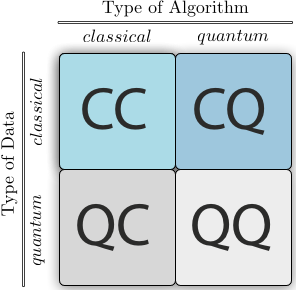
\includegraphics[height=.7\textheight]{Qml_approaches.png}
\end{figure}
Source: \href{https://en.wikipedia.org/wiki/Quantum_machine_learning}{Wikipedia article on Quantum Machine Learning}
\end{frame}

%%%%%%%%%%%%%%%%%%%%%%%%%%%%%%%%%%%%%%%%%%%%%%%%%%%%%%%%%%%%%%%%%%%%%%%
\begin{frame}{Adiabatic quantum optimization}
Solve a nonconvex optimization directly through the adiabatic theorem.
  \begin{itemize}
  	\item Nonconvex objective allows for regularization by 0-1 loss or $l_0$ norm.
  	\item Quantum boosting (\href{https://www.google.com/googleblogs/pdfs/nips_demoreport_120709_research.pdf}{Neven et al., 2009}).
  	\item The possibility is there for a better trade-off between sparsity and accuracy.
  	\item The problem of embedding to the hardware: 
  	\begin{itemize}
  		\item Representation width (1 bit as opposed to the usual 32-bit floating point numbers. It is a form of regularization.
  		\item Limited batch size.
  		\item Embedding the connectivity.
  		\item Finite temperature, inaccuracy of couplings\ldots
  	\end{itemize}
  \end{itemize}
\end{frame}

%%%%%%%%%%%%%%%%%%%%%%%%%%%%%%%%%%%%%%%%%%%%%%%%%%%%%%%%%%%%%%%%%%%%%%%
\begin{frame}{Sampling}
	Gate-based model:
	\begin{itemize}
		\item Quantum deep learning (\href{http://arxiv.org/abs/1412.3489}{Wiebe et al., 2014})
		\begin{itemize}
			\item Learn stacked Boltzmann machines layer by layer.
			\item Uses classical mean-field approximation and efficient state preparation protocol.
		\end{itemize}
	\end{itemize}
	Via annealing:
	\begin{itemize}
		\item Upcoming paper on Meeting 7.
		\item This is how D-Wave is typically used today.
	\end{itemize}
\end{frame}

%%%%%%%%%%%%%%%%%%%%%%%%%%%%%%%%%%%%%%%%%%%%%%%%%%%%%%%%%%%%%%%%%%%%%%
\begin{frame}{Harrow-Hassidim-Lloyd algorithm}
\begin{itemize}
	\item Exponentially faster inversion of well-conditioned matrices (\href{https://arxiv.org/abs/0811.3171}{Harrow et al., 2009}).
	\item Applying it to machine learning started an avalanche.
	\item Quantum support vector machines based on the least-squares formulation (\href{https://arxiv.org/abs/1307.0471}{Rebentrost et al., 2014}).
	\begin{itemize}
		\item Exponential speedup with some caveats.
		\item Sparsity?
	\end{itemize}
	\item For continuous variables, see \href{http://arxiv.org/abs/1603.06222}{Lau et al., 2016}.
\end{itemize}
\end{frame}

%%%%%%%%%%%%%%%%%%%%%%%%%%%%%%%%%%%%%%%%%%%%%%%%%%%%%%%%%%%%%%%%%%%%%%
\begin{frame}{Reinforcement learning in a quantum environment}
\href{https://arxiv.org/abs/1610.08251}{Dunjko et al., 2016}, and coding exercise for \href{https://github.com/peterwittek/qml-rg\#meeting-4}{Meeting 4}.
  \begin{itemize}
    \item What does it even mean that a quantum agent learns? How do we verify that it learned?
    \item Contrast deliberation phase with the deep learning and self-play part of AlphaGo (\href{http://doi.org/10.1038/nature16961}{Silver et al., 2016}).
    \item Result: the best we can hope for is a Grover-like speedup once we start verifying the agent.
  \end{itemize}
\end{frame}

%%%%%%%%%%%%%%%%%%%%%%%%%%%%%%%%%%%%%%%%%%%%%%%%%%%%%%%%%%%%%%%%%%%%%%%
\begin{frame}{Implementations and feasibility}
	\begin{itemize}
		\item Potential photonic implementation with classical tuning of parameters: quantum feedforward networks and autoencoders (\href{https://arxiv.org/abs/1612.01045}{Wan et al., 2016}).
		\item Continuous-variable quantum optics: claimed exponential speedup. (\href{http://arxiv.org/abs/1603.06222}{Lau et al., 2016}).
		\item D-Wave related work, e.g. \href{https://www.google.com/googleblogs/pdfs/nips_demoreport_120709_research.pdf}{Neven et al., 2009}, and an upcoming paper.
		\item \href{http://dx.doi.org/10.1103/physrevlett.114.140504}{Experimental realization of a quantum support vector machine on four qubits} and \href{http://dx.doi.org/10.1088/1367-2630/17/12/123010}{a feasibility study of QRAM}.
	\end{itemize}
\end{frame}

\section{What's Next}
%%%%%%%%%%%%%%%%%%%%%%%%%%%%%%%%%%%%%%%%%%%%%%%%%%%%%%%%%%%%%%%%%%%%%%%
\begin{frame}{The Next Six Meetings}
\begin{columns}[T]
	\begin{column}{.5\textwidth}
	\textbf{Classical}
	 \begin{enumerate}
	  	\item Regularization in deep learning.
	  	\item Sequence learning.
	  	\item Probabilistic graphical models.
	  	\item Generative adversarial networks.
	  	\item Manifold learning\vspace{1.2em}
	  	
	  	\item Recommendation systems and matrix completion.
	  \end{enumerate}
	\end{column}
	\begin{column}{.5\textwidth}
	\textbf{Quantum}
	 \begin{enumerate}
	 	\item Actual quantum Hamiltonian in BMs.
	 	\item Sequential causal models.
	 	\item Quantum graphical models.\vspace{1.2em}
	 	
	 	\item Unidentified quantum whatever topic.
	 	\item Quantum topological analysis.
	 	\item Quantum matrix completion.
	 \end{enumerate}
	\end{column}
\end{columns}
\vspace{1em}

Planned finish date for first phase: 18 May.
\end{frame}

%%%%%%%%%%%%%%%%%%%%%%%%%%%%%%%%%%%%%%%%%%%%%%%%%%%%%%%%%%%%%%%%%%%%%%%
\begin{frame}{Upcoming Tutorials}
\begin{itemize}
	\item Advanced Data Science (18 April).
	\item Kaggle (2 May).
\end{itemize}

The plan afterwards is to replace tutorials by entering a Kaggle competition as a team, with regular meetings.

\end{frame}

\end{document}
